\documentclass[tikz,border=5pt]{standalone}
\usetikzlibrary{calc}
\begin{document}
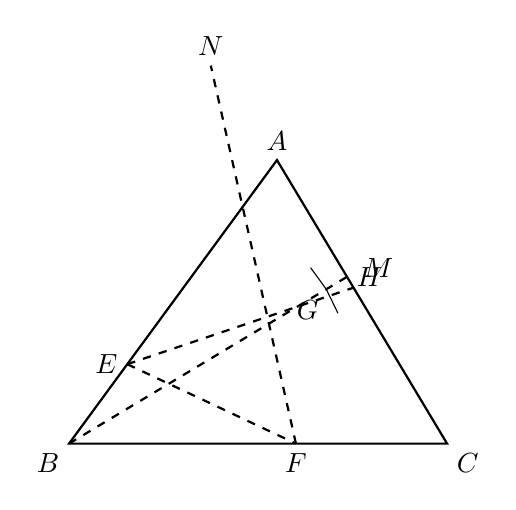
\begin{tikzpicture}[scale=1.2]
  % Main triangle
  \coordinate (B) at (0,0);
  \coordinate (C) at (4,0);
  \coordinate (A) at (2.2,3);
  \draw[thick] (B) -- (C) -- (A) -- cycle;

  % Points
  \coordinate (E) at ($(B)!0.28!(A)$);
  \coordinate (F) at ($(B)!0.6!(C)$);
  \coordinate (M) at ($(A)!0.45!(C)$);
  \coordinate (G) at (intersection of E--M and A--F);
  \coordinate (N) at (1.5,4);

  % Dashed lines
  \draw[dashed,thick] (E) -- (M);
  \draw[dashed,thick] (F) -- (N);
  \draw[dashed,thick] (E) -- (F);

  % Perpendicular from B to line CM (which lies on AC)
  \coordinate (H) at ($(A)!(B)!(C)$);
  \draw[dashed,thick] (B) -- (H);
  % Right angle mark at H
  \draw ($($(H)!8pt!(B)$)!8pt!90:(H)$) coordinate (r1) --
        ($($(H)!8pt!(B)$)!8pt!90:(H)!8pt!90:(B)$) --
        ($(H)!8pt!(B)!8pt!-90:(H)$);

  % Labels
  \node[below left] at (B) {$B$};
  \node[below right] at (C) {$C$};
  \node[above] at (A) {$A$};
  \node[left] at (E) {$E$};
  \node[below] at (F) {$F$};
  \node[above right] at (M) {$M$};
  \node[right] at (G) {$G$};
  \node[above] at (N) {$N$};
  \node[right] at (H) {$H$};
\end{tikzpicture}
\end{document}
